\chapter{Angriffe gegen Machine Learning Anwendungen}\label{sec:angriffe}

Neben den allgemeingültigen Risiken gegen die Informationssicherheit gibt es eine Reihe spezifischer Risiken von Machine Learning Anwendungen.
Im Folgenden werden typische Angriffe gegen Machine Learning Modelle betrachtet und analysiert. 
Der Fokus liegt dabei auf Angriffen, welche besonders das Schutzziel Vertraulichkeit bei Neuronalen Netzen bedrohen.

\section{De-Anonymisierung und Re-Identifikation}

Für Machine Learning Anwendungen werden, je nach Komplexität der Aufgabe, eine Vielzahl an Daten benötigt.
Durch Datenlecks können diese, oftmals private, Daten an die Öffentlichkeit oder in die Hände eines Angreifers gelangen.
Ein Beispiel hierfür wäre das Datenleck von Facebook, bei welchem 50 Millionen Nutzerprofile von dem Datenanalyse-Unternehmen Cambridge Analytica ausgelesen worden sind. 
Diese wurden genutzt, um die US-Wahl 2016 zu beeinflussen \cite{I-2}.

Allerdings kommt es auch vor, dass Unternehmen freiwillig Daten veröffentlichen. 
Netflix veröffentlichte 2006 einen Datensatz, welcher Filmbewertungen von knapp 500.000 Nutzern enthält \cite{I-3}. 
Um nicht absichtlich private Daten zu veröffentlichen, war der Datensatz anonymisiert.
Neben einem Wettbewerb steht dieser Datensatz zu Forschungszwecken öffentlich zur Verfügung.
Narayanan und Shmatikov \cite{P-29} zeigen jedoch, dass die Anonymisierung des Datensatzes nicht ausreichend war, um private Informationen zu schützen.
Die Bewertungen der anonymisierten Benutzer, wurden mit den Bewertungen der öffentlichen Filmdatenbank IMDb abgeglichen.
Dabei genügt es, wenn Präferenzen in Korrelation gesetzt werden können, die genauen Wert sind nicht notwendig.
Narayanan und Shmatikov \cite{P-29} beschreiben, dass sogar politische oder religiöse Informationen herausgefunden werden können.
Hierzu werden beispielsweise positive Bewertungen von religiösen Dokumentationsfilmen, die privat auf Netflix abgegeben werden, werden öffentlichen Profilen auf IMDb zugeordnet.

\section{Property Inference Attacke}\label{sec:property_inference}

Bei der sogenannten Property Inference Attacke versucht ein Angreifer, bestimmte Eigenschaften über die Daten eines Modells herauszufinden, welche nur indirekt von einem Modell gelernt wurden und auch nicht bewusst veröffentlicht wurden \cite{P-80}.

Ateniese et al. \cite{P-80} zeigten erstmals, wie so ein Angriff bei Machine Learning Modellen ,wie einer Support Vektor Maschine, funktionieren kann.
Es wird gezeigt, dass es möglich ist, herauszufinden, ob das angegriffene Modell eine bestimmte Eigenschaft der Daten gelernt hat. 
Um dies zu erreichen, konstruiert der Angreifer mehrere Datensätze, in denen die zu untersuchende Eigenschaft vorhanden ist oder nicht. 
Anschließend werden diese Datensätze genutzt, um verschiedene Modelle zu trainieren, welche die gleiche Architektur wie das angegriffene Modell nachbilden.
Der Schlüssel dieser Methode ist es, nun einen Meta-Klassifikator mit diesen Modellen zu trainieren.
Bei Meta-Klassifikatoren handelt es sich um Modelle, welche aus anderen Modellen lernen. 
Konkret werden hierbei die Parameter der Modelle als Input genutzt, um vorherzusagen, ob die Trainingsdaten die zu untersuchende Eigenschaft besitzen. 
Dies ist möglich, da alle Modelle, das angegriffene Modell und die vom Angreifer trainierten Modelle, die gleiche Architektur haben und dadurch auch zum gleichen Format transformiert werden können.
Ateniese et al. konnten mit diesem Angriff zeigen, dass es möglich ist, herauszufinden, ob ein Sprachmodell mit Daten der Eigenschaft \dq Sprecher mit indischem Dialekt \dq trainiert wurde. 

\begin{figure}[!htb]
    \centering
    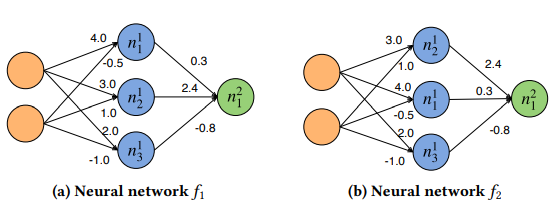
\includegraphics[width=12cm]{figures/permutation_invariance}
    \caption{Permutation eines Neuronalen Netzes \cite{P-11}}
    \label{fig:permutation_invariance}
\end{figure} 

Die Methode von Ateniese et al. \cite{P-80} ist auf diverse Machine Learning Modelle wie Hidden Markov Modelle oder Support Vektor Maschinen ausgelegt, weshalb diese bei Neuronalen Netzen nicht sonderlich gut funktioniert. 
Ganju et al. \cite{P-11} passten den Angriff auf Neuronale Netze an, indem zwei geeignete Repräsentation für diese Art von Modellen genutzt werden kann.
Die erste Repräsentation eines Neuronalen Netz basiert auf der Eigenschaft von Neuronalen Netzen, dass die Reihenfolge der Neuronen vertauscht werden kann. 
Abbildung \ref{fig:permutation_invariance} zeigt zwei Neuronale Netze, bei denen die Reihenfolge der Knoten in der ersten Hidden Layer vertauscht ist, jedoch das Modell die gleiche Funktion berechnet.
Diese Eigenschaft kann nun genutzt werden, um jede Schicht zu sortieren und dadurch eine einheitliche Matrix für Permutationen des gleichen Modells zu erhalten.

Die zweite Repräsentation beruht darauf, die Schichten eines Neuronalen Netzes nicht als Vektor darzustellen.
Im Gegensatz zu einem Vektor hat ein Set keine feste Reihenfolge oder Ordnung, sondern ist lediglich eine Menge von Objekten, bzw. hier von Knoten.
Dies sorgt ebenfalls dafür, dass Permutationen des gleichen Modells, in das gleiche Format übertragen werden können.
Ganju et al. \cite{P-11} zeigen anhand des MNIST Datensatzes, dass beide Repräsentationsformen die Accuracy des Meta-Klassifikators erhöhen können.

Gopinath et al. \cite{P-12} zeigen, dass viele Informationen eines Neuronalen Netzes in der Aktivierung der Neuronen steckt. 
Dabei reicht es, einen Wert in \textbf{on} und \textbf{off} zu unterteilen, wobei on einem Wert > 0 entspricht. 
Gopinath et al. \cite{P-12} nutzten diese Darstellung für eine gutwillige Informationsgewinnung über ein Modell, jedoch könnte die Darstellung auch für Property Inference Angriffe genutzt werden.
\section{Model Inversion Attacke}\label{sec:model_inversion}

Bei der Model Inversion Attacke, versucht ein Angreifer, durch bestimmte Eingaben in ein Modell, Rückschlüsse auf die Trainingsdaten von diesem zu ziehen. 
Dies kann so weit führen, dass einzelne Datensätze nachgebildet werden können \cite{P-3}. 

Fredrikson \etal \cite{P-3} zeigen anhand eines Gesichtserkennungsmodells, dass es möglich ist, das Bild einer Person zu rekonstruieren.
Dabei handelt es sich um einen sogenannten White-Box Angriff.
White-Box bedeutet, dass das Modell vollumfänglich in den Händen des Angreifers ist.
Dies ist beispielsweise der Fall, wenn ein Modell öffentlich geteilt wird.
Eine weitere Voraussetzung ist, dass die zu rekonstruierende Person von dem anzugreifenden Modell klassifiziert werden kann, folglich auch Bilder dieser Person in den Trainingsdaten vorhanden sind.
Abbildung \ref{fig:mi_attacke} zeigt, wie sehr das rekonstruierte Bild (links) dem Originalbild (rechts) ähnelt.

\begin{figure}[!htb]
    \centering
    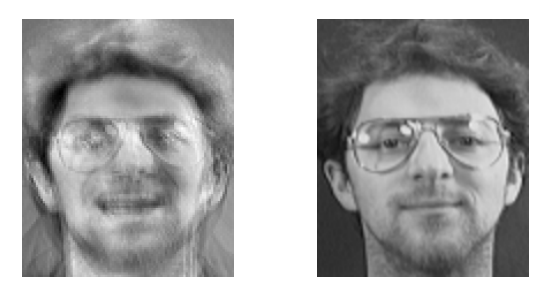
\includegraphics[width=8cm]{figures/mi_attack}
    \caption{Rekonstruktion eines Bildes \cite{P-3}}
    \label{fig:mi_attacke}
\end{figure} 

Der Angriff, auch Reconstruction Attacke genannt, wird durch einen iterativen Algorithmus durchgeführt.
Zu Beginn wird ein initiales Bild, als Startbild gesetzt. 
Hat der Angreifer Hintergrundwissen zu den Daten, so kann er das initiale Bild ähnlich zu dem Zielbild setzen, ansonsten kann es mit festgelegten konstanten Werten oder zufälligen Werten initialisiert werden. 
In jedem Schritt des Algorithmus wird dieses Bild durch das Modell inferiert und anschließend der Wert einer Verlustfunktion bestimmt.
Der Wert dieser ist, sofern das Modell nicht mehr Details zur Vorhersage angibt, lediglich der Wert 1 minus die Wahrscheinlichkeit, auch Confidence Score genannt, ob es sich bei dem eingegebenen Bild um die gesuchte Klasse, auch Label genannt, handelt.
Konkret bedeutet dies, wenn das Bild bereits die zu rekonstruierende Person zeigt, ist der Confidence Score des Labels der Person nahe 1 und damit der Wert der Verlustfunktion nahe 0.
Der Wert der Verlustfunktion kann nun durch das Modell abgeleitet werden und ergibt somit Gradienten für das Bild.
Dies gleicht dem Backpropagation Schritt des Trainings eines neuronalen Netzes, mit dem Unterschied, dass hier das Bild wie ein Teil des Modells behandelt wird und für dieses ebenfalls Gradienten berechnet werden.
Diese Gradienten werden genutzt, um das Bild entgegengesetzt dieser Gradienten anzupassen, sodass der Wert der Verlustfunktion sinkt.
Zusätzlich nutzen die Autoren einen Autoencoder, welcher das angepasste Bild in jedem Schritt harmonisiert und hochskaliert.
Bei diesem Autoencoder handelt es sich um ein neuronales Netz, welches einen Input (hier ein Bild) in einen Vektor mit niedrigerem Rang transformiert und anschließend wieder in einen Vektor mit dem gleichen Rang wie der des Inputs transformiert.
Input und Output eines Autoencoders haben somit den gleichen Rang, hier wird also ein Bild zu einem anderen Bild der gleichen Größe transformiert.
Der Teil des Autoencoders, welcher das Eingabebild in einen Vektor mit niedrigerem Rang transformiert, wird Encoder genannt. 
Der Teil des Autoencoders, welcher das Hochskalieren übernimmt, heißt Decoder.
Zum Training des Autoencoders werden Bilder genutzt, wobei der Input auch gleich dem gewünschten Output entspricht. 
Somit lernt ein Autoencoder, aus einem Bild das gleiche Bild zu erzeugen, jedoch mit der Einschränkung, dass der Vektor innerhalb des Modells einen niedrigen Rang hat.
Folglich ist das erzeugte Bild nicht exakt identisch zu dem eingegebenen Bild.
Der Autoencoder von Fredrikson \etal \cite{P-3} weist jedoch die Besonderheit auf, dass die Eingabebilder verrauscht werden und die gewünschten Ausgabebilder gleich bleiben.
Ziel dadurch ist es, dass der trainierte Autoencoder genutzt werden kann, um unscharfe Bilder zu möglichst scharfen Bildern zu transformieren.
Mit diesem Autoencoder soll also das rekonstruierte Bild nach jeder Iteration schärfer werden und damit näher an dem ursprünglichen Bild liegen.
Die Reconstruction Attacke läuft so lange, bis die maximal konfigurierte Anzahl an Schritten erreicht wird, der Wert der Verlustfunktion einen bestimmten Wert unterschreitet oder sich eine definierte Anzahl an Schritten der Wert der Verlustfunktion nicht reduziert.

Zhang \etal \cite{P-4} erweitern diesen Angriff, indem die Qualität des Autoencoders verbessert wird. 
Der Autoencoder wird nicht nur auf verschwommenen Bildern trainiert, sondern zusätzlich noch auf Bilder, bei welchen jeweils nur ein Bildausschnitt maskiert wird.
Eine weitere Verbesserung besteht darin, zusätzlich ein Modell zu nutzen, welches reale Bilder von synthetischen Bildern unterscheiden soll.
Dieses Konstrukt entspricht dem Diskriminator eines Generative Adversarial Networks \cite{P-86}.
Als Input nutzt dieser Diskriminator Bilder, welche von dem Autoencoder generiert wurden.
Der Wert einer Verlustfunktion des Outputs des Diskriminators kann dabei nicht nur durch den Diskriminator selbst backpropagiert werden, sondern zusätzlich auch noch durch den Autoencoder.
Dies sorgt dafür, dass der Autoencoder ergänzend versucht, möglichst realistische Bilder zu erzeugen.
Mithilfe der zusätzlichen Trainingsdaten und des Diskriminators, wird der Autoencoder verbessert, wodurch die Qualität der einzelnen Bilder erhöht wird und folglich auch die Qualität des rekonstruierten Bildes steigt.
Der restliche Angriff erfolgt simultan zu der bereits beschriebenen Vorgehensweise.
Zhang \etal \cite{P-4} zeigen einen zusätzlichen Angriffsvektor, bei dem ein Angreifer bereits Teile eines Bildes hat. 
Dabei kann es sich um eine verschwommene Version des originalen Bildes handeln, oder um ein Bild, bei dem ein Teil beispielsweise mit einem schwarzen Balken zensiert wird.
Da der Autoencoder zusätzlich mit diesen Fällen trainiert wurde, ist es möglich, die fehlenden Informationen eines Bildes zu ergänzen.



\section{Membership Inference Angriff}\label{sec:membership_inference}

Bei der Membership Inference Attacke versucht ein Angreifer herauszufinden, ob ein Datenpunkt Bestandteil des Trainingsdatensatzes eines Modells ist. 
Dies bedroht die Vertraulichkeit, da beispielsweise herausgefunden werden kann, ob eine bestimmte Person Teil eines Trainingsdatensatzes für die Diagnose einer Krankheit ist und folglich auch mit der entsprechenden Krankheit diagnostiziert ist \cite{P-2}.

Shorki et al. \cite{P-2} führen eine Membership Inference Attacke durch, indem eine Reihe Modelle trainiert wird, die ähnlich dem Angriffsziel-Modell sind.
Diese Modelle werden auch Shadow Modelle genannt.
Ähnlich bedeutet hier, dass sowohl die Funktion der Modelle, als auch der Trainingsdatensatz, mit dem angegriffenen Modell vergleichbar sind.
Einige dieser trainierten Modelle enthalten den zu untersuchenden Datenpunkt im Trainingsdatensatz, andere hingegen nicht.
Nun wird ein binärer Meta-Klassifikator trainiert (analog zu der Property Inference Attacke in Kapitel \ref{sec:property_inference}), welcher anhand der Vorhersagen der Shadow Modelle, Label und Confidence Score, lernt, ob ein Datensatz im Training des entsprechenden Modells genutzt wurde.
Wird in diesen Meta-Klassifikator die Vorhersage des angegriffenen Modells als Input genutzt, so erhält man die Antwort, ob der Datenpunkt für das Modelltraining genutzt wurde oder nicht.
Laut Shorki et al. \cite{P-2} funktioniert dieser Angriff, da ähnliche Modelle, die mit einem ähnlichen Datensatz trainiert wurden, sich auch ähnlich verhalten. 
Somit kann bei den selbst trainierten Modellen, welche den Datensatz enthalten, ein Muster gelernt werden, welches auch auf andere Modelle anwendbar ist. 
Overfitting und eine komplexe Modellarchitektur erhöhen die Wahrscheinlichkeit eines erfolgreichen Angriffs.

Carlini et al. \cite{P-13} zeigen eine Alternative des Angriffs, bei welcher kein Meta-Klassifikator genutzt wurde.
Die Shadow Modelle werden analog zu \cite{P-2} trainiert. 
Anstatt mit den Vorhersagen dieser Modelle nun einen Meta-Klassifikator zu trainieren, werden zwei Gaußverteilungen gebildet, jeweils über die Confidence Scores der Modelle, wo der Datenpunkt im Training enthalten war oder nicht.
Mittels eines Likelihood-Quotienten-Tests wird anschließend vorhergesagt, in welcher Verteilung der Confidence Score des angegriffenen Modells wahrscheinlicher liegt.
Ein Vorteil dieser Methode liegt darin, dass weniger Shadow Modelle trainiert werden müssen, da bereits mit relativ wenig Werten eine Gaußverteilung modelliert werden kann.


Eine Voraussetzung bei Shorki et al. \cite{P-2} ist es, dass der Confidence Score mit ausgegeben wird.
Choquette-Choo et al. \cite{P-7} wandeln den Angriff ab, sodass dieser Score nicht mehr benötigt wird.
Der Angriff funktioniert simultan zu \cite{P-2}, jedoch wird nicht nur der Datenpunkt selber in die Modelle als Input gegeben, sondern auch Abwandlung davon. 
Diese Abwandlungen könnte das Hinzufügen von zufälligem Rauschen sein, oder bei Bilddateien beispielsweise Rotation oder Translation.
Die Hypothese der Autoren ist, dass das Modell bei Datenpunkten, die im Training genutzt wurden, robuster gegenüber diesen Abwandlungen ist und dennoch den Datenpunkt korrekt klassifiziert.
Zusätzlich könnten Abwandlungen der Daten über einen Data Augmentation Schritt auch direkt vom Modell gelernt worden sein.


\section{Data Extraction Attacke}\label{sec:data_ext}

Bei der Data Extraction Attacke versucht ein Angreifer, Informationen eines Modells zu extrahieren, die gelernt wurden, obwohl dies (oftmals) nicht der Fall sein sollte \cite{P-87}.
Der Angriff unterscheidet sich von der Model Inversion Attacke (Kapitel \ref{sec:model_inversion}) und von der Property Inference Attacke (Kapitel \ref{sec:property_inference}), indem Daten direkt aus dem Modell extrahiert werden und nicht anhand der Vorhersage des Modells nachgebildet werden.

Carlini et al. \cite{P-87} beschrieben, dass konkrete Zeichenketten oder Werte, wie eine Kreditkartennummer oder eine Sozialversicherungsnummer, in einem Sprachmodell gelernt werden.
Um dies zu evaluieren, wurde ein Sprachmodell mit dem Penn Treebank Datensatz trainiert, welcher ca. 5MB groß ist. 
Zusätzlich wurde ein Satz eingefügt, welcher mit \textit{\dq My social security number is \dq} beginnt und anschließend eine Zahlenfolge beinhaltet.
Die Funktionalität des Modells liegt darin, das nächste Wort oder Zeichen vorherzusagen, wenn eine Zeichenkette eingegeben wird.
Anzumerken ist hierbei noch, dass dieses Modell signifikant kleiner als 5 MB ist, was folglich bedeutet, dass nicht alle Trainingsdaten in dem Modell gespeichert sein können.
Die Experimente von Carlini et al. \cite{P-87} zeigen, dass dieses Modell die Zahlenfolge ungewollt gelernt hatte als mögliche Vorhersage ausgibt, wenn der oben genannte Satz als Input genutzt wird.

In einem anderen Forschungsprojekt, ebenfalls unter der Leitung von Carlini, \cite{P-88} zeigen die Autoren eine Data Extraction Attacke am Beispiel des Sprachmodells GPT-2. 
Dabei handelt es sich um ein Sprachmodell des Unternehmens OpenAI, welches der Vorgänger von ChatGPT (siehe Kapitel \ref{sec:introduction}) ist und Open Source zur Verfügung steht.
Obwohl voller Zugriff auf das Modell besteht, wird lediglich die Ausgabe des Modells betrachtet. 
Folglich bedeutet dies, dass der Angriff auf jedes Modell anwendbar wäre.
Zur Durchführung des Angriffs wird lediglich ein Starttoken in das Modell eingegeben und anschließend vielfach das vorgeschlagene Folgewort gesammelt. 
Wird dies lang genug gemacht, erhält man eine lange Tokenabfolgen, also quasi Sätze, die vom Modell gelernt wurden. 
Dabei kann es sich um öffentliche Texte handeln, wie beispielsweise der Text der MIT Open Source Lizenz, aber auch private Daten wie Email-Adressen sind vorhanden.
Diese Variation des Angriffs kann in gewissem Maße funktionieren, liefert jedoch oftmals gleiche Wortabfolgen und hat auch eine hohe False-Positive Rate.
Carlini et al. \cite{P-88} variierten deshalb die Methodik, wie die Tokenabfolge gesammelt wird.
Bevor GPT-2 das wahrscheinlichste Folgewort vorschlägt, werden die Wahrscheinlichkeiten in den Wertebereich (0,1) transformiert und so skaliert, dass diese Werte addiert 1 ergeben.
Wird der Softmax Funktion ein Hyperparameter namens Temperatur > 1 mitgegeben, wird das Modell unsicherer und erhöht dadurch die Diversität der Vorhersagen des Modells.
Neben dieser Temperatur wird eine zweite Verbesserung vorgeschlagen. 
Anstatt nur einen Starttoken zu nutzen, werden die ersten Wörter von verschiedenen, öffentlichen Datenquellen genutzt.
Mit diesen zwei Verbesserungen konnten mehr unterschiedliche Arten von Texten, die das Modell gelernt hat, extrahiert werden. 
Neben Newsartikeln oder Forumsbeiträgen, befanden sich auch Kontaktdaten einiger Privatpersonen in diesen Tokenabfolgen.
\section{Poisoning Attacke}\label{sec:poisoning}

Bei der sogenannten Poisoning Attacke werden manipulierte Datensätze in die Trainingsdatenmenge eines Modells injiziert, wodurch das Modell schlechtere oder sogar falsche Vorhersagen trifft.
Ursprünglich ist diese Art des Angriffs recht populär bei Support Vektor Maschinen.
Biggio \etal \cite{P-15} zeigen, dass einige modifizierte Datenpunkte in der Nähe der Entscheidungsgrenze einer Support Vektor Maschine genügen, um die gelernte Funktion deutlich negativ zu beeinflussen.

Yang \etal \cite{P-17} zeigen ein Verfahren, bei dem eine Poisoning Attacke auf neuronalen Netzen angewendet wird.
Ziel hierbei ist es, die gefälschte Daten mit einem absichtlich falschen Label so zu wählen, dass der Wert der Verlustfunktion möglichst groß ist. 
Um dies zu erreichen, wird der Wert der Verlustfunktion des anzugreifenden Modells durch das Modell backpropagiert, wobei die gefälschten Daten als Teil des Modells betrachtet werden. 
Die Daten werden nun in Richtung der Gradienten angepasst, wodurch der Wert der Verlustfunktion steigt.
Werden die gefälschten Daten anschließend genutzt, um das Modell weiter zu trainieren, wird die Verlustfunktionen einen erhöhten Wert aufweisen, was zu einer stärkeren Anpassung des Modells führt, was aufgrund der gefälschten Label zu einer Verschlechterung der Güte des Modells führt.
Um nicht als gefälschte Daten aufzufallen, nutzen Yang \etal \cite{P-17} einen Autoencoder, der Daten so transformiert, dass diese vom Modell als echte Daten erkannt werden.
Damit der Autoencoder lernt, realistische Daten nachzubilden, wird ein zusätzliches Modell genutzt, welches einem Diskriminator der Generative Adversarial Network Architektur \cite{P-86} entspricht.

Guo und Liu \cite{P-16} nutzen einen Ansatz, bei welchem der Angreifer keinen Zugriff auf die Gradienten des angegriffenen Modells braucht.
Stattdessen wird ein vortrainiertes Modell genutzt, welches ähnlich zu dem angegriffenen Modell ist. 
Da diverse Modellarchitekturen Open-Source sind, finden sich auch einige vortrainierte Varianten von diesen im Internet.
Bei Bildklassifikation lässt sich beispielsweise ein vortrainiertes YOLO-Modell nutzen.
Dieses kann dann genutzt werden, um ein generatives Modell zu trainieren, welches wie bei Yang \etal \cite{P-17} die Gradienten des anzugreifenden Modells nutzt, um Daten für das anzugreifende Modell zu verschlimmern.
Guo und Liu \cite{P-16} gehen davon aus, dass das angegriffene Modell noch optimiert wurde und deshalb eine bessere Feature-Erkennung hat, als die öffentlich vortrainierten Modelle.
Dies macht den Angriff effektiver, sofern die Modelle nicht zu unterschiedlich sind.

Poisoning Attacken verschlechtern in der Regel lediglich die Performance eines Modells und sorgen für falsche Vorhersagen.
Tramèr \etal \cite{P-14} zeigen jedoch, dass manipulierte Daten dafür sorgen können, dass andere Angriffe, welche die Vertraulichkeit angreifen, effektiver werden können.
Durch Ändern des Labels eines Datensatzes kann dieser gegebenenfalls zu einem Ausreißer transformiert werden. 
Dadurch passt sich das Modell stärker diesem an, als wenn sich der Datenpunkt in die Messreihe einordnet.
Die falsche Klassifizierung des veränderten Datensatzes würde eine Memberhsip Inferenze Attacke auf diesen verbessern.

\subsection{Verteiltes Lernen}\label{sec:verteiltes_lernen}

Das Verteilte Lernen bietet einige besondere Herausforderungen, die bereits in Kapitel \ref{sec:angriffe_verteiltes_lernen} betrachtet wurden. 
Einige bereits beschriebene Methoden lassen sich problemlos auf das Verteilte Lernen anwenden.
Sollen beispielsweise die Daten der einzelnen Teilnehmer geteilt werden, so ist es möglich, diese mit den Methoden aus Kapitel \ref{sec:aufbereitung_datensatz} vorzuverarbeiten.
Jedoch gibt es auch spezielle Methoden, die auf das Verteilte Lernen ausgerichtet sind.
Im Folgenden werden einige davon genauer beschrieben.

\subsubsection*{Distributed Selective SGD}
Shokri und Shmatikov \cite{P-78} stellen eine Methode vor, bei welcher mehrere Teilnehmer gleichzeitig ein Modell trainieren, ohne dabei die Daten untereinander zu teilen.
Diese wird Distributed Selective Stochastic Gradient Descent oder auch Distributed Selective SGD genannt.
Das Modell liegt dabei auf einem zentralen Server.
Bei der ersten Iteration laden die Teilnehmer das gesamte Modell herunter, bei weiteren Iterationen nur eine festgelegte Anzahl der am meisten geupdateten Parametern (Gewichte).
Dadurch soll vermieden werden, dass Overfitting auf den Daten eines einzelnen Teilnehmers auftritt.
Die heruntergeladenen Parameter ersetzen die alten Parameter an der entsprechenden Stelle im lokalen Modell.
Anschließend wird dieses lokale Modell mit den eigenen Daten trainiert und im Nachhinein eine festgelegte Menge an Gradienten übertragen. 
Diese können dabei entweder randomisiert ausgewählt werden, oder möglichst nach Größe sortiert werden.
Alle Teilnehmer wählen die zu teilenden Gradienten mit der gleichen Strategie aus und behalten diese über den Trainingsprozess bei.
Zusätzlich ist es möglich, die Gradienten vor dem Teilen noch mit in der Größe zu begrenzen oder Rauschen mittels Differential Privacy hinzuzufügen.
Abbildung \ref{fig:dssgd} zeigt die Architektur von Distributed Selective SGD.

\begin{figure}[!htb]
    \centering
    \includegraphics[width=12cm]{figures/dssgd}
    \caption{Distributed Selective SGD \cite{P-78}}
    \label{fig:dssgd}
\end{figure} 

Durch das eingeschränkte Teilen der Gradienten werden so wenig Information wie nötig geteilt, jedoch ist die Güte des Modells kaum schlechter als bei normalem Training.
Die Autoren begründen dies damit, dass das lokale Modell lokale Minima durch das Ersetzen von Parametern aus dem geteilten Modell verlassen kann und so weiter eher Richtung globales Minimum konvergiert. 
Zwei Parameter steuern dabei die Performance des Modells beim Training mit Distributed Selective SGD: das Privacy Budget $\epsilon$ und die Anzahl der zu teilenden Gradienten.
Werden mehr Gradienten nach jedem Schritt von jedem Teilnehmer geteilt, kann das Privacy Budget $\epsilon$ niedriger angesetzt werden, um dennoch eine nahezu identische Güte im Vergleich zu einem normal trainierten Modell zu erhalten.

\subsubsection*{Anspruchsvolle kryptografische Methoden}

Takabi et al. \cite{P-104} nutzen Homomorphe Verschlüsselung, um ein Modell zu trainieren, welches Daten von mehreren Teilnehmern nutzen kann. 
Die Funktionsweise der Methode mit einem Teilnehmer wurde bereits in Kapitel \ref{sec:homomorphe_verschlüsselung} beschrieben.
Diese lässt sich problemlos auf mehrere Teilnehmer erweitern, indem abwechselnd Daten jedes Teilnehmers verschlüsselt an den Server übertragen wird und diese für das Training des Modells mittels Homomorpher Verschlüsselung genutzt wird.
Da Daten jeweils verschlüsselt sind, ist es nicht möglich, Daten anderer Teilnehmer zu extrahieren.

Auch das auf Funktionaler Verschlüsselung basierende Framework CryptoNN \cite{P-53}, welches in Kapitel \ref{sec:funktionale_verschlüsselung} vorgestellt wurde, kann für Verteiltes Lernen genutzt werden. 
Die Rolle des Clients können dabei mehrere Teilnehmer übernehmen, wohingegen die Autorität jedoch von einem separaten System übernommen werden muss. 
Anschließend können auch bei dieser Methode abwechselnd Daten von verschiedenen Teilnehmern zum Trainieren genutzt werden.

Ein weiterer Ansatz für Verteiltes Lernen, welches auf Funktionaler Verschlüsselung basiert, wurde von Xu et al. \cite{P-33} mit dem Namen HybridAlpha vorgestellt.
Ähnlich zu dem bereits beschriebenen CryptoNN Framework, gibt es auch eine Autorität, welche die benötigten kryptografischen Schlüssel an die Server und Clients verteilt.
Jedoch übertragen die Clients keine Daten an den Server, sondern trainieren ein lokales Modell.
Die aktualisierten Modellparameter werden anschließend mit Differential Privacy verrauscht und dann verschlüsselt an den Server übertragen.
Hat der Server alle verschlüsselten Modellparameter jedes Teilnehmers gesammelt, wird mittels Funktionaler Verschlüsselung die Summe der Gewichte jedes Neurons gebildet.
Daraus kann der Server anhand der Anzahl an Teilnehmern, den Durchschnittswert für jedes Gewicht jedes Neurons bilden und aktualisiert damit das globale Modell.
Die Autoren zeigen anhand des MNIST Datensatze \cite{D-MNIST}, dass die Güte eines Modells, welches mit HyrbidAlpha ohne Differential Privacy trainiert wurde, sehr nahe der Güte eines Modells ist, welches in einem Verteilten Lernen Szenario ohne HyrbidAlpha gelernt wurde. 
Wird jedoch zusätzlich Differential Privacy genutzt, sinkt die Güte des Modells. 
Mit einem Privacy Budget von $\epsilon=0,5$ sinkt die Genauigkeit der Klassifikation um knapp 10\%.


\subsubsection*{Secure Multi-Party Computation}

Bei der Secure Multi-Party Computation handelt es sich um einen Forschungsbereich mit dem Ziel, dass Teilnehmer gemeinsam eine Funktion berechnen können, ohne dass die einzelnen Eingabewerte aufgedeckt werden. 
Methoden dieses kryptografischen Forschungsgebiets können auch für Neuronale Netze genutzt werden.

Rouhani et al. \cite{P-71} stellten ein Framework namens DeepSecure vor, welches Oblivious Transfer, zu Deutsch vergessliche Übertragung, und Garbled Circuits, zu Deutsch verdrehte Schaltkreise, nutzt.
Oblivious Transfer ist ein kryptografisches Protokoll zwischen einem Sender und einem Empfänger, bei dem der Empfänger einen Index zwischen 1 und $n$ auswählt und der Sender die Nachricht mit dem entsprechenden Index übermittelt. 
Der Sender weiß dabei jedoch nicht, welcher Index ausgewählt wurde.
Diese Methodik wird auch 1-aus-$n$ Oblivious Transfer genannt.
Garbled Circuits, auch Yao's Garbled Circuits genannt, ist ebenfalls ein Protokoll, bei der eine Funktion als Boolescher Schaltkreis mit zwei Eingabegattern dargestellt wird.
Dabei erstellt einer der beiden Teilnehmer, hier Alice genannt, Wahrheitstabellen zu jedem Logikgatter des Schaltkreises. 
Die Inputs sind dabei nicht 0 und 1, sondern jeweils eine Folge von $k$ randomisierten Bits, welche 0 und 1 kodieren.
Die Ergebnisspalte dieser Wahrheitstabellen verschlüsselt Alice anschließend mit den beiden Inputs, sodass dies nur mit den beiden Inputs wieder entschlüsselt werden kann. 
Zusätzlich wird die Reihenfolge der Zeilen randomisiert, damit aufgrund der Reihenfolge keine Rückschlüsse gewonnen werden können. 
Dieser Schritt wird Garbling genannt und die entstandenen Tabellen sind sogenannte Garbled Tabellen.
Anschließend überträgt Alice die Garbled Tabellen an den zweiten Teilnehmer, hier Bob.
Mittels 1-aus-2 Oblivious Transfer wählt Bob eine von zwei Nachrichten aus, wobei der Index seinem Input entspricht und die zwei Nachrichten die kodierten Labels von Alice sind.
Die erhaltene Nachricht und das eigene Label können nun genutzt werden, um die Ergebnisspalte einer Garbled Tabelle zu entschlüsseln.
Bob führt dies für jedes Gatter des Schaltkreises aus.
Am Ende erhält Bob den Output des letzten Gatters, welchen jedoch einer der randomisierten Bitfolgen ist. 
Er übermittelt diesen an Alice und erhält dadurch den entsprechenden 0 oder 1 Wert.
DeepSecure wendet Garbled Circuits auf Neuronale Netze an.
Alice würde in diesem Fall die Daten besitzen und Bob das Modell, welches trainiert wird.
Der Feedforward Schritt würde dabei durch einen Booleschen Schaltkreis aus XOR und XNOR Gattern implementiert werden, wodurch die Berechnung der Vorhersage erfolgt.
Dadurch kann Bob den Wert der Verlustfunktion und anschließend der Gradienten bestimmen, ohne die Daten von Alice zu kennen.
Alice würde jedoch auch nicht die genauen Gewichte des Modells kennen.
Allerdings ist die Anzahl an benötigten Gattern, um ein Neuronales Netz darzustellen, enorm.
Einige Operationen, wie die Anwendung einer Aktivierungsfunktion, benötigt mehrere tausende Gatter.
Jedes dieser Gatter sorgt ebenfalls dafür, dass eine Menge an Daten übertragen werden muss.
Ein Neuronales Netz, welches $28\times28$ Pixel Bilder als Input nimmt, zwei Hidden Layers mit 300 und 100 Knoten (Sigmoid Aktivierungsfunktion) besitzt und eine Softmax Output Layer mit 10 Knoten hat, würde circa 171.300.000 Gatter ausmachen und in einem Feedforward Schritt ungefähr 2 Gigabyte an Daten übertragen.

\subsubsection*{Aggregation}
Eine alternative Methode wird von Bonawitz et al. \cite{P-36} vorgestellt.
Diese basiert auf sicherer Aggregation, welche mehrere Daten von unterschiedlichen Teilnehmern verbindet, ohne dass die Daten eines einzelnen Teilnehmers erkenntlich werden.
Teilnehmer trainieren ein lokales Modell mit den eigenen privaten Daten. 
Bevor die angepassten Parameter aber an das globale Modell übertragen werden, werden die Parameter mit den Parametern anderer Teilnehmer kryptografisch aggregiert.
Dadurch erhält das globale Modell Gradienten aller Trainingsdaten, ohne die einzelnen Daten zu kennen.


%\section{Weitere Angriffe}

Neben den bereits beschriebenen Angriffe, gibt es noch einige zusätzliche Angriffe, wo jedoch nicht die Vertraulichkeit der Daten im Visier des Angreifers liegt. 
Für die Vollständigkeit dieses Kapitels, werden einige relevante Angriffe dennoch erwähnt.
Weiterentwicklungen oder Abwandlungen könnten in Zukunft dennoch Einfluss auf die Vertraulichkeit der Daten haben, so wie es bereits bei der Poisoning Attacke in Kapitel \ref{sec:poisoning} beschrieben wurde.

\subsection{Evasion Attack}



\subsection{Backdoor Attack}